\chapter{Data import via ODBC}
\label{chap:odbc}

Since version 1.7.5, \app{gretl} provides a method for retrieving data
from databases which support the ODBC standard. Most users
won't be interested in this, but there may be some for whom this
feature matters a lot: typically, those who work in an environment
where huge data collections are accessible via a Data Base Management
System (DBMS).

ODBC is the \emph{de facto} standard for interacting with such
systems. In the next section we provide some background information on
how ODBC works. What you actually need to do to have \app{gretl}
retrieve data from a database is explained in
section~\ref{sec:odbc-syntax}.

\section{ODBC base concepts}
\label{sec:odbc-base}

ODBC is short for \emph{Open DataBase Connectivity}, a group of
software methods that enable a \emph{client} to interact with a
database \emph{server}. The most common operation is when the client
fetches some data from the server. ODBC acts as an intermediate layer
between client and server, so the client ``talks'' to ODBC rather than
accessing the server directly (see Figure~\ref{fig:odbc}).

\begin{figure}[htbp]
  \centering
  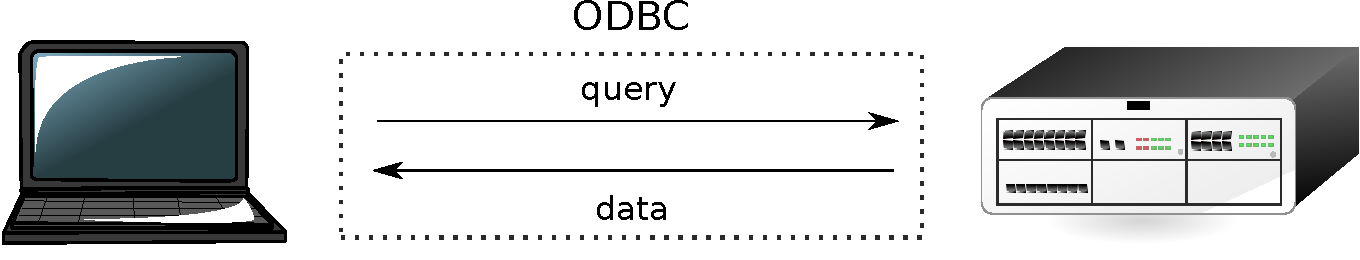
\includegraphics[width=0.8\textwidth]{figures/odbc}
  \caption{Retrieving data via ODBC}
  \label{fig:odbc}
\end{figure}

For the above mechanism to work, it is necessary that the relevant
ODBC software is installed and working on the client machine (contact
your DB administrator for details). At this point, the database (or
databases) that the server provides will be accessible to the client
as a \emph{data source} with a specific identifier (a Data Source Name
or DSN); in most cases, a username and a password are required to
connect to the data source.

Once the connection is established, the user sends a \emph{query} to
ODBC, which contacts the database manager, collects the results and
sends them back to the user. The query is almost invariably formulated
in a special language used for the purpose, namely SQL.\footnote{See
  \url{http://en.wikipedia.org/wiki/SQL}.} We will not provide here an
SQL tutorial: there are many such tutorials on the Net; besides, each
database manager tends to support its own SQL dialect so the precise
form of an SQL query may vary slightly if the DBMS on the other end is
Oracle, MySQL, PostgreSQL or something else.

Suffice it to say that the main statement for retrieving data is the
\texttt{SELECT} statement.  Within a DBMS, data are organized in
\emph{tables}, which are roughly equivalent to spreadsheets. The
\texttt{SELECT} statement returns a subset of a table, which is itself
a table. For example, imagine that the database holds a table called
``NatAccounts'', containing the data shown in
Table~\ref{tab:odbc-nataccounts}.

\begin{table}[htbp]
  \centering
  \begin{tabular}{rrrrr}
    \hline
    year	& qtr	& gdp	 & consump	& tradebal \\ 
    \hline
    1970	& 1	& 584763 & 344746.9	& $-$5891.01 \\ 
    1970	& 2	& 597746 & 350176.9	& $-$7068.71 \\ 
    1970	& 3	& 604270 & 355249.7	& $-$8379.27 \\ 
    1970	& 4	& 609706 & 361794.7	& $-$7917.61 \\ 
    1971	& 1	& 609597 & 362490	& $-$6274.3  \\ 
    1971	& 2	& 617002 & 368313.6	& $-$6658.76 \\ 
    1971	& 3	& 625536 & 372605	& $-$4795.89 \\ 
    1971	& 4	& 630047 & 377033.9	& $-$6498.13  
  \end{tabular}
  \caption{The ``NatAccounts'' table}
  \label{tab:odbc-nataccounts}
\end{table}

The SQL statement
\begin{code}
  SELECT qtr, tradebal, gdp FROM NatAccounts WHERE year=1970;
\end{code}
produces the subset of the original data shown in Table~\ref{tab:odbc-result}.

\begin{table}[htbp]
  \centering
  \begin{tabular}{rrrrr}
    \hline
    qtr	& tradebal & gdp    \\ 
    \hline
    1	& $-$5891.01 & 584763 \\ 
    2	& $-$7068.71 & 597746 \\ 
    3	& $-$8379.27 & 604270 \\ 
    4	& $-$7917.61 & 609706  
  \end{tabular}
  \caption{Result of a \texttt{SELECT} statement}
  \label{tab:odbc-result}
\end{table}

\app{Gretl} provides a mechanism for forwarding your query to the DBMS
via ODBC and including the results in your currently open dataset.

\section{Syntax}
\label{sec:odbc-syntax}

At present, ODBC import is only possible via the command line
interface.\footnote{Since designing a graphical interface for this is
  conceptually simple but rather time-consuming, what we're aiming at
  is a robust and reasonably powerful implementation of the data
  transfer. Once all the issues are sorted out, we'll start
  implementing a GUI interface.} The two commands that gretl uses at
present for fetching data via an ODBC connection are \texttt{open} and
\texttt{data}.

The \texttt{open} command is used for connecting to a DBMS: its syntax
is
\begin{flushleft}
\texttt{%
  open dsn=\emph{database} [user=\emph{username}]
  [password=\emph{password}] --odbc
}
\end{flushleft}
The \texttt{user} and \texttt{password} items are optional; the effect
of this command is to initiate an ODBC connection. It is assumed that
the machine \app{gretl} runs on has a working ODBC client installed.

In order to actually retrieve the data, the \texttt{data} command is
used. Its syntax is:
\begin{flushleft}
\texttt{%
  data \emph{series} [obs-format=\emph{format-string}] \emph{query-string} --odbc
}
\end{flushleft}
where:
\begin{description}
\item[\emph{series}] is the name of the gretl series to contain the
  incoming data, which needs not exist prior to the query. Note that
  the \texttt{data} command imports one series at a time.
\item[\emph{format-string}] is an optional parameter, used to handle
  cases when a ``rectangular'' organisation of the database cannot be
  assumed (more on this later);
\item[\emph{query-string}] is a string containing the SQL statement
  used to extract the data.
\end{description}

The \texttt{\emph{query-string}} can, in principle, contain any valid
SQL statement which results in a table: a ``\texttt{;}'' character at
the end will be added automatically. This string may be specified
directly within the command, as in
\begin{code}
  data x "SELECT foo FROM bar" --odbc
\end{code}
which will store into the gretl variable \texttt{x} the content of the
column \texttt{foo} from the table \texttt{bar}. However, since in a
real-life situation the string containing the SQL statement will be
rather long, it may be best to create it just before the call to
\texttt{data}. For example:
\begin{code}
  string SqlQry = "SELECT foo FROM bar"
  data x SqlQry --odbc
\end{code}

If the optional parameter \texttt{obs-format} is absent, as in the
above example, the SQL query should return \emph{exactly one} column
of data, which is used to fill the variable \texttt{x}
sequentially.  It may be necessary to include a \texttt{smpl} command
before the \texttt{data} command to set up the right ``window'' for
the incoming data.  In addition, if one cannot assume that the data
will be delivered in the correct order (typically, chronological
order), the SQL query should contain an appropriate \texttt{ORDER BY}
clause.

The optional format string is used for those cases when there is no
certainty that the data from the query will arrive in the same order
as the \app{gretl} dataset. This may happen when missing values are
interspersed within a column, or with data that do not have a natural
ordering, e.g.\ cross-sectional data. In this case, the SQL statement
should return a table with $n$ columns, where the first $n-1$ columns
are used to identify which observation the value in the $n$-th column
belongs to. The format string is used to translate the first $n-1$
fields into a string which matches the string \app{gretl} uses to
identify observations in the currently open dataset. At present, $n$
should be between 2 and 4, which should cover most, if not all, cases.

For example, consider the following fictitious case: we have a
5-days-per-week dataset, to which we want to add the stock index for
the Verdurian market;\footnote{See
  \url{http://www.almeopedia.com/index.php/Verduria}.} it so
happens that in Verduria Saturdays are working days but Wednesdays are
not. We want a column which does \emph{not} contain data on
Saturdays, because we wouldn't know where to put them, but at the same
time we want to place missing values on all the Wednesdays.

In this case, the following syntax could be used
%
\begin{code}
  string QRY="SELECT year,month,day,VerdSE FROM AlmeaIndexes"
  data y obs-format="%d/%d/%d" @QRY --odbc
\end{code}
%
The column \texttt{VerdSE} holds the data to be fetched, which will go
into the \app{gretl} series \texttt{y}. The first three columns are
used to construct a string which identifies the day. Since a string
like \texttt{"2008/04/26"} does not correspond to any observation in
our dataset (it's a Saturday), that row is simply discarded. On the
other hand, since no string \texttt{"2008/04/23"} was found in the
data coming from the DBMS (it's a Wednesday), that entry is left blank
in our variable \texttt{y}.

\section{Examples}
\label{sec:examples}

\begin{table}[htbp]
  \centering
  \begin{tabular}{p{0.4\textwidth}p{0.4\textwidth}}
  Table \texttt{Consump} &
  Table \texttt{DATA} \\
    
\begin{tabular}{ll}
\hline
 Field   & Type           \\ 
\hline 
 time    & decimal(7,2)   \\ 
 income  & decimal(16,6) \\ 
 consump & decimal(16,6) \\
\hline
\end{tabular} &

\begin{tabular}{ll}
\hline
 Field   & Type           \\ 
\hline 
 year    & decimal(4,0)  \\ 
 qtr     & decimal(1,0)  \\ 
 varname & varchar(16)   \\ 
 xval    & decimal(20,10)\\ 
\hline
\end{tabular}

  \end{tabular}

  \caption{Example AWM database -- structure}
  \label{tab:odbc-AWMexample1}
\end{table}

\begin{table}[htbp]
  \centering
  \begin{tabular}{p{0.475\textwidth}p{0.475\textwidth}}
  Table \texttt{Consump} &
  Table \texttt{DATA} \\
    
\begin{tabular}{lll}
  1970.00	& 424278.975500	& 344746.944000 \\ 
  1970.25	& 433218.709400	& 350176.890400 \\ 
  1970.50	& 440954.219100	& 355249.672300 \\ 
  1970.75	& 446278.664700	& 361794.719900 \\ 
  1971.00	& 447752.681800	& 362489.970500 \\ 
  1971.25	& 453553.860100	& 368313.558500 \\ 
  1971.50	& 460115.133100	& 372605.015300 \\ 
\ldots \\ 
\end{tabular} &

\begin{tabular}{lllr}
1970	& 1	& CAN	& $-$517.9085000000\\ 
1970	& 2	& CAN	& 662.5996000000 \\ 
1970	& 3	& CAN	& 1130.4155000000\\ 
1970	& 4	& CAN	& 467.2508000000 \\ 
1970	& 1	& COMPR	& 18.4000000000  \\ 
1970	& 2	& COMPR	& 18.6341000000  \\ 
1970	& 3	& COMPR	& 18.3000000000  \\ 
1970	& 4	& COMPR	& 18.2663000000  \\ 
1970	& 1	& D1	& 1.0000000000   \\ 
1970	& 2	& D1	& 0.0000000000   \\ 
\ldots \\ 
\end{tabular}
\end{tabular}
  \caption{Example AWM database --- data}
  \label{tab:odbc-AWMexample2}
\end{table}

In the following examples, we will assume that access is available to
a database known to ODBC with the data source name ``AWM'', with
username ``Otto'' and password ``Bingo''. The database ``AWM''
contains quarterly data in two tables (see \ref{tab:odbc-AWMexample1}
and \ref{tab:odbc-AWMexample2}):

The table \texttt{Consump} is the classic ``rectangular'' dataset;
that is, its internal organization is the same as in a spreadsheet or
in an econometrics package like \app{gretl} itself: each row is a data
point and each column is a variable. On the other hand, the structure
of the \texttt{DATA} table is different: each record is one figure,
stored in the column \texttt{xval}, and the other fields keep track of
which variable it belongs to, for which date.

\begin{script}[htbp]
  \caption{Simple query from a rectangular table}
  \label{ex:odbc-1}
\begin{scode}
nulldata 160
setobs 4 1970:1 --time
open dsn=AWM user=Otto password=Bingo --odbc

string Qry1 = "SELECT consump FROM Consump"
data cons @Qry1 --odbc

string Qry2 = "SELECT income FROM Consump"
data inc @Qry2 --odbc
\end{scode}
\end{script}

Example \ref{ex:odbc-1} shows two elementary queries: first we set up
an empty quarterly dataset. Then, we connect to the database by the
\texttt{open} statement. Once the connection is established we
retrieve, one column at a time, the data from the \texttt{Consump}
table. In this case, no observation string is necessary because the
data are already arranged in a matrix-like structure, so we only need
to bring over the relevant columns.

\begin{script}[htbp]
  \caption{Simple query from a non-rectangular table}
  \label{ex:odbc-2}
\begin{scode}
string S = "select year, qtr, xval from DATA \
       where varname='WLN' ORDER BY year, qtr"
data wln obs-format="%d:%d" @S --odbc
\end{scode}
\end{script}

In example \ref{ex:odbc-2}, on the contrary, we make use of the
observation string, since we are drawing data from the \texttt{DATA}
table, which is not rectangular. The SQL statement stored in the
string \texttt{S} produces a table with three columns. The
\texttt{ORDER BY} clause ensures that the rows will be in
chronological order, although this is not strictly necessary in this
case.

\begin{script}[htbp]
  \caption{Handling of missing values for a non-rectangular table}
  \label{ex:odbc-3}
\begin{scode}
string foo = "select year, qtr, xval from DATA \
       where varname='STN' AND qtr>1"
data bar obs-format="%d,%d" @foo --odbc
print bar --byobs
\end{scode}

Example \ref{ex:odbc-3} shows what happens if the rows in
the outcome from the \texttt{SELECT} statement do not match the
observations in the currently open \app{gretl} dataset. The query
includes a condition which filters out all the data from the first
quarter. The query result (invisible to the user) would be something
like
\begin{code}
+------+------+---------------+
| year | qtr  | xval          |
+------+------+---------------+
| 1970 |    2 |  7.8705000000 | 
| 1970 |    3 |  7.5600000000 | 
| 1970 |    4 |  7.1892000000 | 
| 1971 |    2 |  5.8679000000 | 
| 1971 |    3 |  6.2442000000 | 
| 1971 |    4 |  5.9811000000 | 
| 1972 |    2 |  4.6883000000 | 
| 1972 |    3 |  4.6302000000 | 
...
\end{code}
Internally, \app{gretl} fills the variable \texttt{bar} with the
corresponding value if it finds a match; otherwise, \texttt{NA} is
used. Printing out the variable \texttt{bar} thus produces
\begin{code}
     Obs           bar

  1970:1              
  1970:2        7.8705
  1970:3        7.5600
  1970:4        7.1892
  1971:1              
  1971:2        5.8679
  1971:3        6.2442
  1971:4        5.9811
  1972:1              
  1972:2        4.6883
  1972:3        4.6302
...
\end{code}

\end{script}
